\documentclass[conference]{IEEEtran}
%future work: local patch operator
%complexity
\usepackage{bigstrut}
\usepackage{balance}
\usepackage{subfig}
\usepackage{wrapfig}
\usepackage{amsmath}
\usepackage{hyperref}
\usepackage{pifont}
\usepackage{mdframed}
\pagenumbering{gobble}
\usepackage{lettrine}
\usepackage{placeins}
%\usepackage{times}
\usepackage{rotating}
\usepackage{booktabs}
%\usepackage{balance} 
\usepackage{color, colortbl}
\usepackage{graphicx}
\usepackage{algorithmicx}
\usepackage[running]{lineno}
\usepackage{times}
\usepackage{fancyhdr,graphicx,amsmath,amssymb}
\usepackage[ruled,vlined]{algorithm2e}
\include{pythonlisting}
\usepackage{program}
\usepackage{cite}
\usepackage{alltt}
\usepackage{balance}
\newcommand{\eq}[1]{Equation~\ref{eq:#1}}
\newcommand{\bi}{\begin{itemize}}
	\newcommand{\ei}{\end{itemize}}
\newcommand{\be}{\begin{enumerate}}
	\newcommand{\ee}{\end{enumerate}}
\newcommand{\tion}[1]{\textsection\ref{sec:#1}}
\newcommand{\fig}[1]{Figure~\ref{fig:#1}}
\definecolor{lightgray}{gray}{0.975}
\usepackage{fancyvrb}
\usepackage{float}
\usepackage{stfloats}
\usepackage{multirow}
\usepackage{listings}
\usepackage{amsmath}  
\DeclareMathOperator*{\argmin}{arg\,min} 
\DeclareMathOperator*{\argmax}{arg\,max} 
%\usepackage[usenames]{xcolor}
\bibliographystyle{unsrt}



\usepackage{color}
\newcommand{\colorrule}[1]{\begingroup\color{#1}\hrule\endgroup}

\definecolor{darkgreen}{rgb}{0,0.3,0}

\usepackage[table]{xcolor}
\definecolor{Gray}{rgb}{0.88,1,1}
\definecolor{Gray}{gray}{0.85}
\definecolor{Blue}{RGB}{0,29,193}
\newcommand{\G}{\cellcolor{green}}
\newcommand{\Y}{\cellcolor{yellow}}
\newcommand{\tc}{\centering\arraybackslash}
\newcommand\topspace{\rule{0pt}{2.6ex}}       % Top strut
\newcommand{\stack}[3]{\vskip 1mm\shortstack{Min : #1 \\ Med : #2 \\ Max : #3}}


\definecolor{MyDarkBlue}{rgb}{0,0.08,0.45} 
\newenvironment{changed}{\par\color{MyDarkBlue}}{\par}

\newcommand{\ADD}[1]{\textcolor{MyDarkBlue}{{\bf #1}}}
\newcommand{\addit}[1]{\begin{changed}\input{#1}\end{changed}}

\usepackage{color}
\usepackage{listings}
\usepackage{setspace}

\usepackage{array}
\newcolumntype{$}{>{\global\let\currentrowstyle\relax}}

\newcolumntype{^}{>{\currentrowstyle}}
\newcommand{\rowstyle}[1]{\gdef\currentrowstyle{#1}%
  #1\ignorespaces
}

\lstnewenvironment{python}[1][]{
\lstset{
	mathescape,
	numbers=right,
	numberstyle=\scriptsize,
	stepnumber=1,
	numbersep=0.5em,
	xleftmargin=0em,
	framextopmargin=2em,
	framexbottommargin=2em,
	showspaces=false,
	showtabs=false,
	showstringspaces=false,
	tabsize=2,
	% Basic
	basicstyle=\ttfamily\scriptsize\setstretch{0.8},
	backgroundcolor=\color{Background},
	language=Python,
	% Comments
	commentstyle=\color{Comments}\slshape,
	% Strings
	stringstyle=\color{Strings},
	morecomment=[s][\color{Strings}]{"""}{"""},
	morecomment=[s][\color{Strings}]{'''}{'''},
	% keywords
	morekeywords={[1]import,from,class,def,for,while,if,is,in,elif,else,not,and,or,print,break,continue,return,True,False,None,access,as,,del,except,exec,finally,global,import,lambda,pass,print,raise,try,assert, dot, norm, zip, sorted},
	keywordstyle={[1]\color{Code}\bfseries},
	% additional keywords
	morekeywords={[3]fastmap,Slope,bPruning,clister,train,leafs,weightedFeatures,HOW, exemplar,nearestSlope,dist,displace,geometry,splitAcross2Points,leaves,How,nearest,bPruning,Stats,divide,recurse,weight1,project, furthest, split,WHERE,clusterer, getContours,envied, fWeight, nearestContour, projection, mutate, HERE, knn},
	keywordstyle={[3]\color{Keywords}\bfseries},
	morekeywords={[2]@invari},
	keywordstyle={[2]\color{Decorators}\slshape},
	emph={self},
	emphstyle={\color{self}\slshape},
	firstnumber=last
	%
}}{}


\definecolor{Gray}{gray}{0.9}
\definecolor{Gray}{gray}{0.95}
\newcommand{\kw}[1]{\textit{#1}}
\newcommand{\quart}[4]{\begin{picture}(80,6)
	{\color{black}\put(#3,3){\circle*{2.5}}\put(#1,3){\line(1,0){#2}}}\end{picture}}

% New Commands
\usepackage{etex}
\author{Rahul Krishna, George Mathew\\
	Computer Science, North Carolina State University, USA\\
	\{rkrish11, george2\}\@ncsu.edu
}
\title{Evolutionary Multi-Objective Optimization:\\ A Distributed Computing approach}
% \usepackage{etoolbox}
\makeatletter
\makeatother


\pagestyle{plain}
\begin{document}
	\maketitle
	\begin{abstract}
		Multi-objective problems are usually complex, NP-Hard, and resource intensive. Although exact methods can be used, they consume prohibitively large amounts of time and memory. An alternative approach would be to make use of meta-heuristic algorithms, which approximate the Pareto frontier in a reasonable amount of time. Even so, these meta-heuristic algorithms consume a significant amount of time. 
		
		Parallel and distributed computing used in design and implementation of these algorithms may offer significant speed-ups. In addition to this, they may be used to improve the quality, increase the robustness of the the obtained solutions, and may also allow the algorithms to be scaled to solve large problems. 
		
		We present parallel models for two multi-objective optimization problems: Diffential Evolution(DE) and Geometric Active learner(GALE).
		
	\end{abstract}
	\begin{IEEEkeywords}
		Evolutionary Algorithms, Multi Objective Optimization, Parallelization, Pareto Frontier
	\end{IEEEkeywords}
	
	\section{Introduction} 
	
	\lettrine{M}{etaheuristic} search methods such as Evolutionary Algorithms are commonly used to \textit{optimize} many real-world applications \cite{89genetic,storn97}. Optimization is the task of finding solutions which satisfy one or more specified objectives. There are two types of optimizers, a single-objective optimization involves a single objective function and a single solution, a multi-objective optimization considers several objectives simultaneously. In case of a multi-objective optimizer generates a set of alternate solutions with certain trade-offs. These are called Pareto optimal solutions. 
	
	The design of the evolutionary algorithms naturally leads to parallelization. They contain several individuals which are being improved through generations. This parallel nature is particularly useful when implementing the algorithm on distributed systems. Many real-world applications have time consuming function evaluations and therefore parallelizing the evaluations on a set of available computing resources speeds up the optimization task. In addition to this, steady advances in new technologies such as Grid Computing \cite{abramson2000nimrod} allows parallelization to be performed with relative ease. Several Parallel Evolutionary Algorithms have been studied in the literature (e.g., in \cite{alba2002parallelism,branke2004distribution,deb2003distributed}). 
	
	There are several parallel computing strategies (models) \cite{08parallel}, here we explore the three main models --- the Island model, Master-Slave model and Diffusion model. The current focus of this paper is the Island model, where the population for a given run is divided into semi-isolated subpopulations. Each subpopulation is assigned to a separate processor of the parallel computing system. The run begins with the one-time random creation of a separate population of individuals at each processor of the parallel computer system.
	
	In this project, we aim to present parallel models for two evolutionary multi-objective optimizers: (1) Differential Evolution (DE) \cite{storn97}; and (2) Geometric Active Learning (GALE) \cite{krall15}. For implementation, we use the \textit{henry2 Linux cluster} offered by NC State with message passing (OpenMPI)~\cite{openMPI04} a distributed programming environment.
	
	This report is organized as follows. The following section presents a brief background on the pertinent topics. In \textsection\ref{algos}, we discuss various strategies for parallelization. In \textsection\ref{experiments}, we provide our experimental results. \textsection\ref{problem} we discuss the problems we are studying followed by the parallelization strategies in \textsection\ref{strategies}. In \textsection\ref{experiments} and \textsection\ref{results} we describe our experiments and discuss the results. \textsection\ref{conclusion} summarizes the conclusions we can draw from the experiments. Finally, \textsection\ref{future} highlights our work can be enhanced.
	
	\section{Evolutionary Algorithms}
	\label{algos}
	An Evolutionary Optimization(EO) begins its search with a population of solutions usually created at random within a specified lower and upper bound on each variable. If bounds are not supplied in an optimization problem, suitable values can be assumed only for the initialization purpose. Thereafter, the EO procedure enters into an iterative operation of updating the current population to create a new population by the use of four main operators: selection, crossover, mutation and elite-preservation. The operation stops when one or more termination criteria are met. The two main EO we plan to study are listed below:
	
	\subsection{Differential Evolution (DE)} 
	
	The Differential Evolution algorithm involves maintaining a population of candidate solutions subjected to iterations of recombination, evaluation, and selection. The recombination approach involves the creation of new candidate solution components based on the weighted difference between two randomly selected population members added to a third population member. This perturbs population members relative to the spread of the broader population. In conjunction with selection, the perturbation effect self-organizes the sampling of the problem space, bounding it to known areas of interest on the Pareto frontier. \fig{de} highlights the algorithmic details of the algorithm.
	
	\begin{figure}[h]
		\begin{mdframed}
			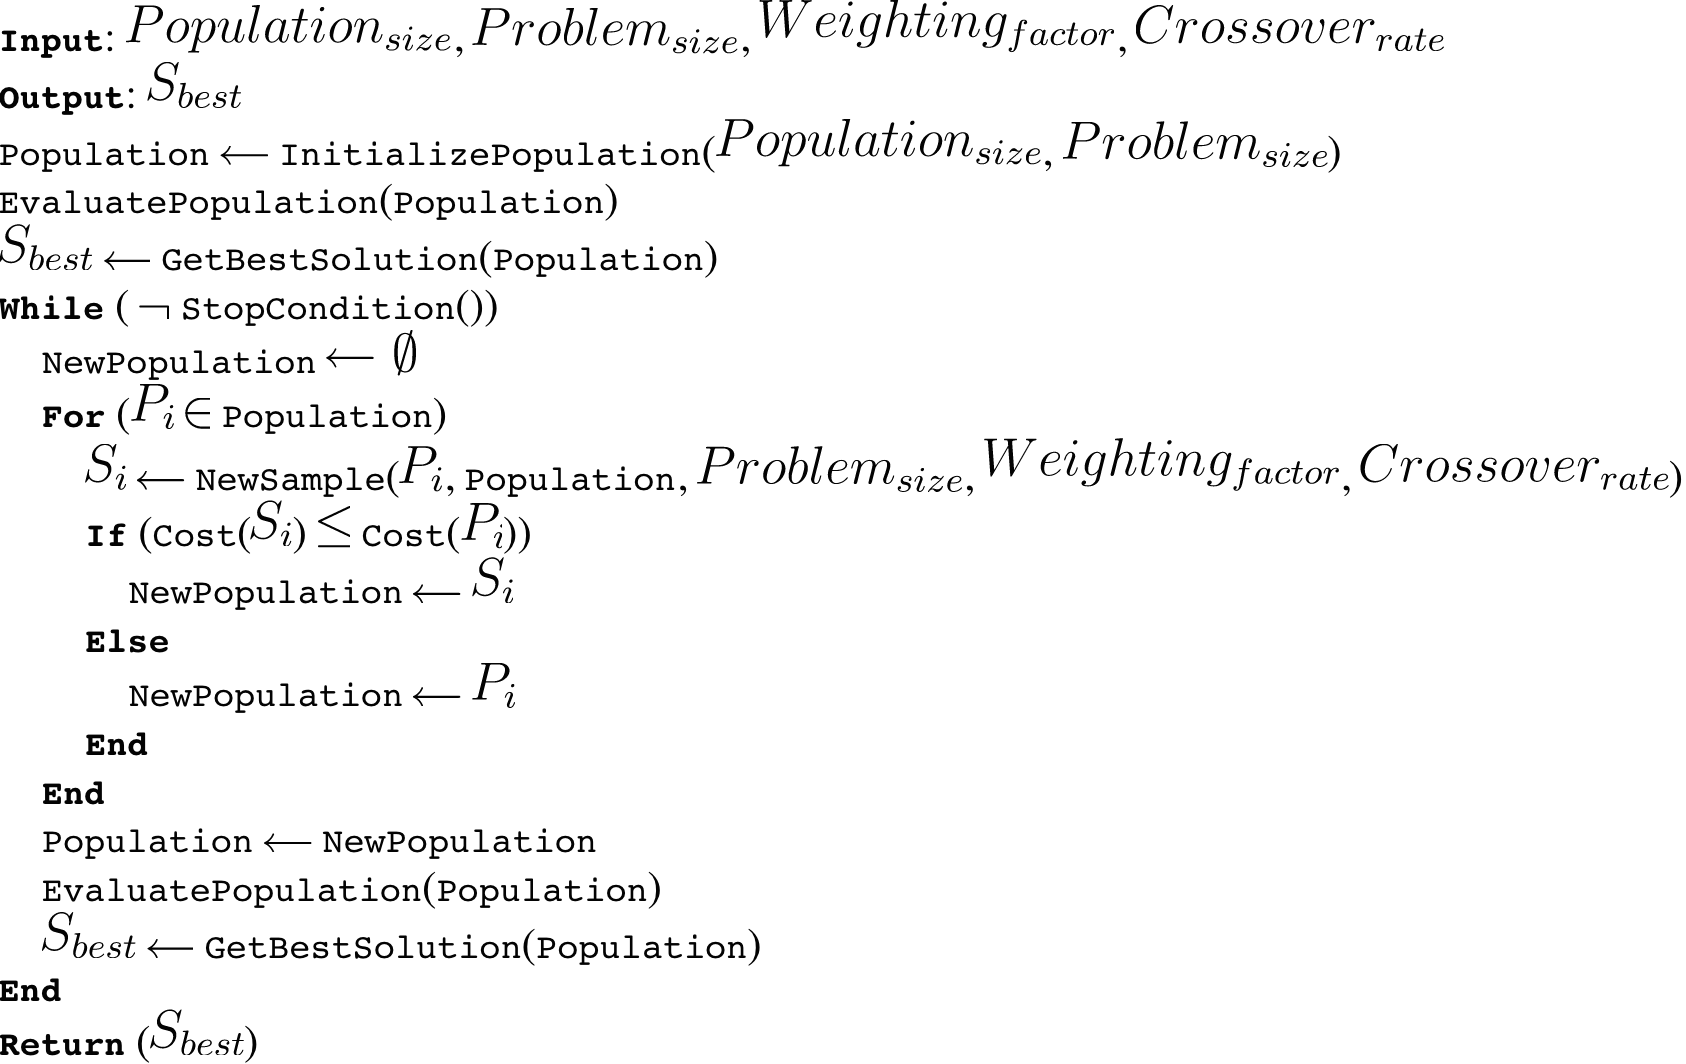
\includegraphics[width=\linewidth]{img/de.png}
		\end{mdframed}
		\caption{Algorithm: Differential Evolution}	
		\label{fig:de}
	\end{figure}
	
	
	\subsection{Geometric Active Learning (GALE)} 
	
	GALE is a near-linear time multi-objective optimization algorithm that builds a piecewise approximation to the surface of best solutions along the Pareto frontier. GALE uses a recursive hierarchical clustering algorithm called WHERE, which is powered by a FASTMAP \cite{faloutsos95}, to recursively reduce the dimensions to a single principal component, see \fig{where}. After clustering, the non dominated leaf is identified(i.e the leaf with the best set of solutions) and all the points within this leaf cluster is mutated along the principal component to generate a subset of the population for the next generation. The rest of the population is randomly generated over the decision space. GALE uses only the poles(extreme points in a cluster) to check for domination. This reduces the number of evaluations drastically and improves the performance for models that takes significant time to evaluate a set of decisions.
	
	\begin{figure}
		\begin{mdframed}[backgroundcolor=white]
			
			{\bf Top-down Clustering with WHERE}
			
			WHERE  divides data into  groups of size $\alpha=\sqrt{N}$. 
			Using this measure, WHERE runs as follows:
			\begin{enumerate}[leftmargin=3mm]
				\item Find   two   distance cases,  $X,Y$
				by picking any case $W$ at random, then setting $X$ to its most
				distant case, then setting $Y$ to the case most distant from
				$X$
				(which requires only $O(2N)$ comparisons).
				\item Project each case $Z$
				to position $x$ on a    lines running from $X$ to $Y$: if $a,b$  are distances  $Z$ to $X,Y$  then  $x = (a^2+c^2 - b^2)/(2ac)$.
				\item Split the data at the median $x$ value of all cases.
				\item For   splits larger than  $\alpha=\sqrt{N}$, recurse from step1.
			\end{enumerate}
			In terms of related work,
			the above is similar in approach to Boley's PDDP algorithm~\cite{boley98}, but PDDP requires an $O(N^2)$ calculation
			at each recursive level to find the PCA principle component. Our method, on the other hand,
			performs the same task with only $O(2N)$ distance calculations 	using the 
			FASTMAP heuristic~\cite{Faloutsos1995} shown in step1. Platt~\cite{platt05} notes that FASTMAP is a  Nystr\"om approximation to the first component of PCA.  
		\end{mdframed}
		\caption{Algorithm: WHERE}
		\label{fig:where}
	\end{figure}
	
	\begin{figure}[t!]
		\centering
		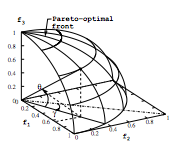
\includegraphics{img/dtlz2_pareto.png}
		\caption{Pareto Frontier of DTLZ2}
		\label{fig:problem}
	\end{figure}
	
	\begin{figure}
	\centering
	{\footnotesize \begin{tabular}{lr}
		\hline
		\rowcolor[gray]{.9} Setting & Value \\ \hline
		Population Size               & 100   \\
		Number of Generations         & 100   \\
		Mutation Rate                 & 0.75  \\ 
		Crossover Probability         & 0.3  \\ \hline
	\end{tabular}}
	\caption{Settings for DE}
	\label{fig:de_settings}
	\vspace{5mm}
	{\footnotesize \begin{tabular}{lr}
		\hline
		\rowcolor[gray]{.9} Setting & Value \\ \hline
		Population Size               & 100   \\
		Number of Generations         & 100   \\
		Domination Factor             & 0.15  \\ \hline 
	\end{tabular}}
	\caption{Settings for GALE}
	\label{fig:gale_settings}
	\end{figure}
	

	
	\begin{figure}
	\centering
	{\footnotesize \begin{tabular}{>{\tc}m{0.81in} >{\tc}m{0.8in} >{\tc}m{0.62in}}
	\hline
	\rowcolor[gray]{.9}Algorithm & Convergence & Diversity \\ \hline
	DE(Serial) & \stack{1.80e-5}{2.23e-5}{2.56e-5} & \stack{0.37}{0.44}{0.54} \\ \hline 
	DE(Parallel) & \stack{1.80e-5}{2.25e-5}{2.58e-5} & \stack{0.38}{0.43}{0.49} \\ \hline 
	GALE(Serial) & \stack{5.28e-4}{5.49e-4}{5.73e-4} & \stack{0.36}{0.41}{0.49} \\ \hline 
	GALE(Parallel) & \stack{5.273-4}{5.54e-4}{5.78e-4} & \stack{0.39}{0.42}{0.51} \\ \hline 
	\end{tabular}}
	\caption{Range of Results for optimizers}
	\label{fig:results_table}
	\end{figure}
	
	
	\section{Optimization Problem}
	\label{problem}
	
	Multi-objective Evolutionary Algorithms(MOEA) require scalable test problems that help test its efficiency. 
	
	\subsection{DTLZ2}
	\label{dtlz2}
	\textbf{DTLZ2} is a mathematical test problem \cite{debMOEA02}, which was formulated by \textit{Kalyanmoy \textbf{D}eb}, \textit{Lothar \textbf{T}hiele}, \textit{Marco \textbf{L}aumans} and \textit{Eckhart \textbf{Z}itzler}. 
	
	\textbf{Decisions} : DTLZ2 has 30 decisions between 0 and 1.
	\[0 \leq {x}_{i} \leq 1 \ \ \ \ where \ \  i = 1,2 ,3 .... 30\]
	
	\textbf{Objectives} : Although DTLZ2 allows as to generate upto n-1 objectives where n is the number of decisions, we choose to limit the number of objectives to 3 since we can model the objectives better to visualize the pareto frontier. Limiting the number of objectives also controls the domination pressure. All the three objectives needs to be minimized. The objectives are defined as follows:
	\[{f}_{1}(x) = (1+g({x}_{M}))\cos({x}_{1} \pi/2)....\cos({x}_{M-1} \pi/2)\]
	\[{f}_{2}(x) = (1+g({x}_{M}))\cos({x}_{1} \pi/2)....\cos({x}_{M-1} \pi/2)\]
	\[{f}_{3}(x) = (1+g({x}_{M}))\sin({x}_{1} \pi/2)\]
	\[where \ \ \ \ g({x}_{M}) = \sum_{x \in {x}_{M}} (x_i - 0.5)^2 \]
	
	\textbf{Optimal Solutions} : The pareto optimal solutions corresponds to the decisions \(x_i = 0.5\) and all objective function values must satisfy \(\sum_{m=1}^M (f_m)^2 = 1\). Figure \ref{fig:problem} shows the pareto frontier that represents the optimal solutions of DTLZ2.
	
	\subsection{POM3}
	\label{pom3}
	POM3 is a simulation of requirement prioritization strategies proposed by \textbf{P}ort, \textbf{O}klov and \textbf{M}enzies\cite{boehm03POM}. POM3 has 9 decisions and its possible values are described in table \ref{fig:pom3_decisions}. POM3 has 4 objectives.
	
	\begin{itemize}
	\item \textbf{Cost :} Cost of completing the project. To be \textbf{\textit{minimized}}.
	\item \textbf{Utility :} Normalized Utility of the project. To be \textbf{\textit{maximized}}.
	\item \textbf{Completion Percentage :} Expected percentage of project that can be completed. To be \textbf{\textit{maximized}}.
	\item \textbf{Idle Time :} Total unproductive time of developers. To be \textbf{\textit{minimized}}. 
	\end{itemize}
	
	\begin{table}[t]
	    \centering
		\begin{tabular}{ll}
			\hline
			\rowcolor[HTML]{EFEFEF} 
			\multicolumn{1}{l}{\cellcolor[HTML]{EFEFEF}{\bf Decision}} & \multicolumn{1}{c}{\cellcolor[HTML]{EFEFEF}{\bf  Range}}  \\ \hline
			\rowcolor[HTML]{FFFFFF} 
			{\bf Culture}  & $0.10<x<0.90$\\
			\rowcolor[HTML]{FFFFFF} 
			{\bf Criticality} & $0.82<x<1.26$\\
			\rowcolor[HTML]{FFFFFF} 
			{\bf Criticality Modifier} & $0.02<x<0.10$\\
			\rowcolor[HTML]{FFFFFF} 
			{\bf Initial Known} & $0.40<x<0.70$\\
			\rowcolor[HTML]{FFFFFF} 
			{\bf Inter-Dependency} & $0.0<x<1.0$\\
			\rowcolor[HTML]{FFFFFF} 
			{\bf Dynamism} & $1.0<x<50.0$\\
			\rowcolor[HTML]{FFFFFF} 
			{\bf Size} & $x \in [3,10,30,100,300]$\\
			\rowcolor[HTML]{FFFFFF} 
			{\bf Team Size} & $1.0<x<44.0$\\
			\rowcolor[HTML]{FFFFFF} 
			{\bf Plan} & $0<x<4$\\
		\end{tabular}
		\caption{Decisions for POM3}
		\label{fig:pom3_decisions}
	\end{table}
	
	
	\subsection{XOMO}
	\label{xomo}
	XOMO is a Monte Carlo Simulator which models NASA's space program software\cite{menzies05xomo}. XOMO has 23 decisions and are described in figure \ref{fig:xomo_decisions}. XOMO has 4 objectives all of which have to be minimized.
	
	\begin{itemize}
	\item \textbf{Effort :} Total effort required by the developer to complete the project.
	\item \textbf{Months :} Total number of months required to complete the project.
	\item \textbf{Defects :} Total number of ``bugs" in the project.
	\item \textbf{Risk :} Risk involved in completing the project.
	\end{itemize}
	
	\begin{figure*}[htbp]
    \begin{minipage}{\linewidth}
        \centering
        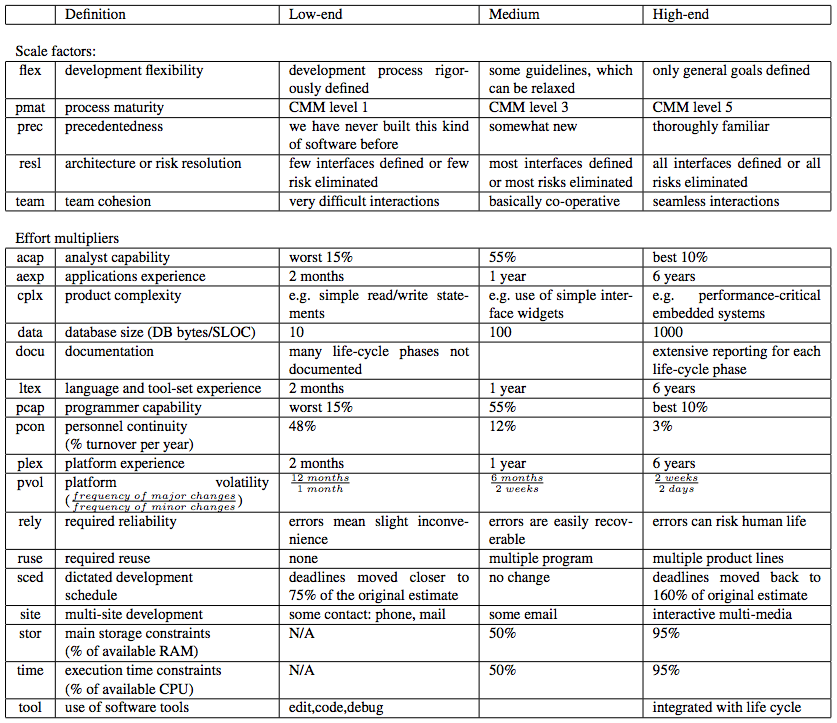
\includegraphics[width=\linewidth]{img/XOMO_decisions.png}
		\caption{Decisions for XOMO}
		\label{fig:xomo_decisions}
    \end{minipage}
    \end{figure*}
    
    \subsection{ERS}
    \label{ers}
    \textbf{E}mergency \textbf{R}esponse \textbf{S}ystem (ERS) is a software feature model\footnote{\url{https://en.wikipedia.org/wiki/Feature_model}}. A feature model is a compact representation of all the products of the Software Product Line in terms of ``features". Feature models are visually represented by means of feature diagrams. Parent and Child features are categorized as 
    \begin{itemize}
	\item \textbf{Mandatory :} Child feature is required.
	\item \textbf{Optional :} Child feature is optional.
	\item \textbf{Or :} Atleast one of the sub-features must be selected.
	\item \textbf{Alternative :} One of the sub-features must be selected.
	\end{itemize}
	
	ERS contains 35 decisions and 3 objectives.
	
	\section{Measures}
	\label{measures}
	The accuracy and effectiveness of the parallelization strategies are indicated by some mathematical measures. We use 4 such evaluation metrics in our experiments and it is highlighted in Figure \ref{fig:measure}.
	
	
	\begin{figure}[!htb]
		\begin{tabular}{ll}
			\hline
			\rowcolor[HTML]{EFEFEF} 
			\multicolumn{1}{l}{\cellcolor[HTML]{EFEFEF}{\bf Measure}} & \multicolumn{1}{c}{\cellcolor[HTML]{EFEFEF}{\bf  Description}}  \\ \hline
			\rowcolor[HTML]{FFFFFF} 
			{\bf Runtime}  & \begin{tabular}[l]{@{}l@{}}Time taken for the algorithm to be gener-\\ate optimal solutions.\end{tabular}\\\hline
			\rowcolor[HTML]{FFFFFF} 
			{\bf Speed Up}  & \begin{tabular}[l]{@{}l@{}}Ratio of time taken for the parallelized \\ version of the algorithm over the time\\taken for the serial version.\end{tabular}\\\hline
			\rowcolor[HTML]{FFFFFF} 
			{\bf Convergence}  & \begin{tabular}[l]{@{}l@{}}Convergence represents the accuracy of \\the obtained solutions. It is the distance\\between the obtained solutions and ideal\\Pareto frontier.\end{tabular}\\\hline
			\rowcolor[HTML]{FFFFFF} 
			\hline{\bf Diversity}                                           & \begin{tabular}[l]{@{}l@{}}Diversity represents the spread of the\\proposed solutions. Ideally the solutions\\should be well distributed across the Par-\\eto frontier,rather than concentrated in\\certain regions.\end{tabular}\\ \hline
		\end{tabular}
		\caption{Performance Measures}
		\label{fig:measure}
	\end{figure}
	
	\section{Parallelization Strategies}
	\label{strategies}
	\subsection{Island Model}
	\label{island}
	In the ``island" approach to parallelization of genetic programming\cite{gustafson2006speciating}, the population for a given run is divided into semi-isolated subpopulations (called demes). Each sub-population is assigned to a separate processor of the parallel computing system. The run begins with the one-time random creation of a separate population of individuals at each processor of the parallel computer system. Each processor runs an instance of the optimizer on the sub-population and the final sub-population across each processor is aggregated and represents the approximate Pareto Frontier. This algorithm takes advantage of the randomness of the optimizer in mutation and achieves similar results to optimizing a population on a single processor.
	
	\subsection{Master Slave Model}
	\label{masterSlave}
	The Master slave model of parallelization uses one processes as a master and all the remaining processors as slaves for optimization\cite{rutkowski13Master}. For each generation of optimization, the master selects a sub-population for each free slave processor. The size of the sub-population is  equal to size of the population divided by the number of slaves. The slave evaluates the fitness and computes the best solution(s) for each population set. The slave then mutates the sub-population and sends the mutants and the evaluations back to the master. The master aggregates results from all the slaves and repeats until the number of generations are completed.
	
	\section{Experimental Setup}
	\label{experiments}
	Python is our choice of programming language. This is due to its support for efficient computation frameworks like numpy\footnote{\url{http://www.numpy.org}} and scipy\footnote{\url{http://www.scipy.org}} that enables quick prototyping and benchmarking.
	For parallelization,  we used the OpenMPI implementation of the Message Passing Interface over a python wrapper and the ``multiprocessing"\footnote{\url{https://docs.python.org/2/library/multiprocessing.html}} package of python. The Open MPI Project\footnote{\url{http://www.openmpi.org}} is an open source Message Passing Interface implementation that is developed and maintained by a consortium of academic, research, and industry partners.The parallelized version of the algorithm could be deployed on HPC to measure the efficiency of the algorithm. The \textit{henry2}\footnote{\url{https://ncsu.edu/hpc/}} shared memory linux cluster by NCSU may be used for this purpose. These nodes provide up to 16 shared memory processor cores and up to 128GB of memory accessible through a dedicated queue. 
	
	For our experiments to evaluate the convergence and diversity, we used 4 cores using 128 GB of shared memory. To evaluate the runtimes and speedup, the experiments were conducted on 1 to 16 cores with 128 GB of shared memory. The parameters we use for Differential Evolution and GALE are shown in \ref{fig:de_settings} and \ref{fig:gale_settings} respectively.
	
	
	\section{Results}
	\label{results}
	
	\subsection{Accuracy}
	The results for runtime, convergence and diversity are shown in \ref{fig:results_table}. Each optimizer is run over a random initial sample of the population 20 times to get the range of output values. The values in the 20 iterations are shown as bar charts representing the median and inter-quartile range of the 20 runs in \fig{results_table}.  As we can see the serialized version of DE yields the lowest convergence. The diversity for all three optimizers are in the same range.
	
	
	To provide a more comprehensive comparison, we studied the optimizers and ranked them statistically. To do this we made use of the Scott-Knott procedure recommended by Mittas \& Angelis\cite{mittas13}. This method
	sorts a list of $l$ treatments with $ls$ measurements by their median
	score. It then
	splits $l$ into sub-lists $m,n$ in order to maximize the expected value of
	differences  in the observed performances
	before and after divisions. E.g. for lists $l,m,n$ of size $ls,ms,ns$ where $l=m\cup n$:
	\[E(\Delta)=\frac{ms}{ls}abs(m.\mu - l.\mu)^2 + \frac{ns}{ls}abs(n.\mu - l.\mu)^2\]
	Scott-Knott then applies some statistical hypothesis test $H$ to check
	if $m,n$ are significantly different. If so, Scott-Knott then recurses on each division.
	
	As a example, consider the following hypothetical data collected under different treatments {\em rx}:
	
	{\scriptsize \begin{verbatim}
		rx1 = [0.34, 0.49, 0.51, 0.6]
		rx2 = [0.6,  0.7,  0.8,  0.9]
		rx3 = [0.15, 0.25, 0.4,  0.35]
		rx4=  [0.6,  0.7,  0.8,  0.9]
		rx5=  [0.1,  0.2,  0.3,  0.4]
		\end{verbatim}}
	\noindent
	After sorting and division, Scott-Knott declares:
	\bi
	\item Ranked \#1 is rx5 with median= 0.25
	\item Ranked \#1 is rx3 with median= 0.3
	\item Ranked \#2 is rx1 with median= 0.5
	\item Ranked \#3 is rx2 with median= 0.75
	\item Ranked \#3 is rx4 with median= 0.75
	\ei
	Note that Scott-Knott found  little
	difference between rx5 and rx3. Hence,
	they have the same rank, even though their medians differ.
	
	Scott-Knott is better than an 
	all-pairs hypothesis test of all methods; e.g. six treatments
	can be compared \mbox{$(6^2-6)/2=15$} ways. 
	A 95\% confidence test run for each comparison has  a very low total confidence: 
	\mbox{$0.95^{15} = 46$}\%.
	To avoid an all-pairs comparison, Scott-Knott only calls on hypothesis
	tests {\em after} it has found splits that maximize the performance differences.
	
	For this study, our hypothesis test $H$ was a
	conjunction of the A12 effect size test of  and
	non-parametric bootstrap sampling; i.e. our
	Scott-Knott divided the data if {\em both}
	bootstrapping and an effect size test agreed that
	the division was statistically significant (99\%
	confidence) and not a ``small'' effect ($A12 \ge
	0.6$).
	
	
	
	\begin{figure}[t]
		{\scriptsize \begin{tabular}{l@{~~~}l@{~~~}l@{~~~}l@{~~~}c}
			\arrayrulecolor{darkgray}
			\hline
			\rowcolor[gray]{.9}  Rank & Optimizer & Median & IQR & 
			%min= 20, max= 117
			\bigstrut\\ \hline
			1 &      DE(Parallel) &    2.30$\times10^{-5}$  &  2.74$\times10^{-6}$ & \quart{1}{1}{1}{100} \bigstrut\\
			1 &      DE(Serial) &    2.36$\times10^{-5}$  &  3.04$\times10^{-6}$ & \quart{1}{1}{1}{100} \bigstrut\\
			\hline
			
			2 &      GALE(Serial) &    5.49$\times10^{-4}$  &  8.72$\times10^{-6}$ & \quart{70}{1}{71}{100} \bigstrut\\
			2 &       GALE(Parallel) &    5.54$\times10^{-4}$  &  2.21$\times10^{-5}$ & \quart{70}{10}{76}{100} \bigstrut\\ \hline
			
		\end{tabular}}
		\caption{Convergence of Optimizers. }\label{fig:convergence}
		\vspace{0.25cm}
		{\scriptsize \begin{tabular}{llllcc}
			\arrayrulecolor{darkgray}
			\hline 
			\rowcolor[gray]{.9}  Rank & Optimizer & Median & IQR & & 
			%min= 20, max= 117
			\bigstrut\\ \hline
			1 &      GALE(Parallel) &    0.416  &  0.070 & \quart{45}{6}{47}{100} & \bigstrut\\ 
			1 &      DE(Parallel) &    0.417  &  0.049 & \quart{45}{4}{47}{100} & \bigstrut\\ 
			1 &      DE(Serial) &    0.431  &  0.056 & \quart{46}{5}{48}{100} & \bigstrut\\
			1 &      GALE(Serial) &    0.432  &  0.047 & \quart{46}{4}{48}{100} &\bigstrut\\ \hline
			
		\end{tabular}}
		\caption{Diversity of Optimizers. }\label{fig:diversity}
	\end{figure}
			
	We have estimated the Scott-Knott rankings for convergence and diversity for all three of the optimizer methods. We did not estimate it for runtime since DE was almost 50 times faster than GALE, hence there was no statistical significance to measure it.
	
	From figure \ref{fig:convergence} we can see that the serialized version of DE produces the best result with rank 1, but there is no statistical difference between the serialized and parallel version of GALE in terms of convergence. The black dot in the last column shows the median value of convergence over 20 runs and the line shows the set of values between the 25th and 75th percentile. We can see that the variance for convergence is very small for all the optimizers, since the inter-quartile distance between the 25th and 75th quartile is almost 0.
	
	The figure \ref{fig:diversity} shows that there is no statistical difference in diversity between all the three methods.
	
	\subsection{Performance}
	
	HPC supports upto 16 processors with 128GB of shared memory. Speed up of a processor is calculated as
	
	\[SpeedUp = \frac{{T}_{Serial}}{{T}_{Parallel}} \]
	
	where ${T}_{Serial}$ is the time taken to run the optimizer on a single processor and ${T}_{n}$ is the time taken to run the optimizer parallely on \textbf{n} number of processors where n varies from 2 to 16.
	
	\begin{figure*}[htbp]
    \begin{minipage}{0.98\linewidth}
        \centering
        \begin{tabular}{$l@{\hspace{6pt}} $l@{\hspace{12pt}} *{9}{^c@{\hspace{10pt}}}}
        \toprule
        \rowstyle{\bfseries\boldmath} STRATEGY & \rowstyle{\bfseries\boldmath} MODEL  & 1 & 2 & 4 & 6 & 8 & 10 & 12 & 14 & 16\\
        \midrule
        \bfseries Island & \bfseries GALE
        & 96.38
        & 50.32
        & 25.92
        & 17.98
        & 13.17
        & 10.56
        & 9.14 
        & 7.67 
        & 6.97 \\
        \bfseries Island & \bfseries DE
        & 0.97
        & 0.53
        & 0.23
        & 0.15
        & 0.11
        & 0.08
        & 0.14
        & 0.09
        & 0.06 \\
        \bfseries Master-Slave & \bfseries GALE
        & 68.3
        & 18.16
        & 4.92
        & 2.38
        & 1.59
        & 1.25
        & 0.99
        & 0.91
        & 0.86 \\
        \bfseries Master-Slave & \bfseries DE
        & 4.05
        & 1.43
        & 0.61
        & 0.31
        & 0.22
        & 0.18
        & 0.14
        & 0.12
        & 0.14 \\
        \bottomrule
        \end{tabular}
        \caption{Runtimes of DTLZ-2 using GALE and DE in seconds}
        \label{tab:DTLZ2_runtimes}
    \end{minipage}
    \begin{minipage}{0.5\linewidth}
    \centering
    \begin{mdframed}
		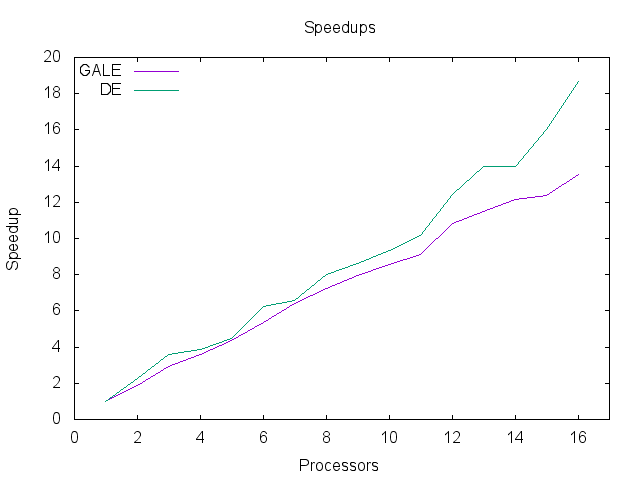
\includegraphics[width=\linewidth]{img/island/dtlz2/speedups}
	\end{mdframed}
	\caption{Island Model DTLZ2 Speed Ups}	
	\label{fig:DTLZ2_island_speedups}
    \end{minipage}
    \begin{minipage}{0.5\linewidth}
    \centering
    \begin{mdframed}
		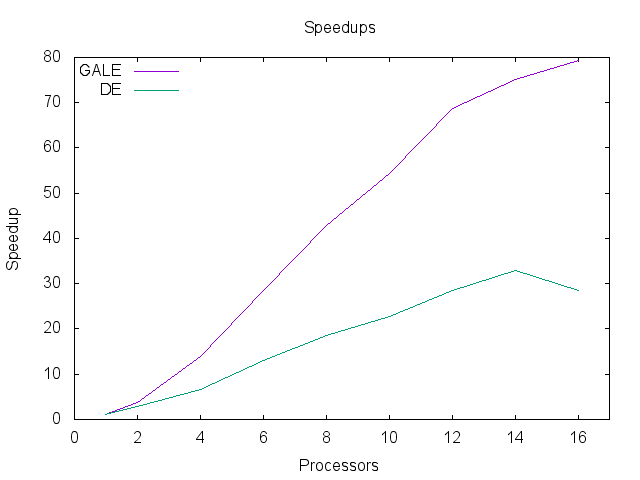
\includegraphics[width=\linewidth]{img/master-slave/dtlz2/speedups}
	\end{mdframed}
	\caption{Master Slave Model DTLZ2 Speed Ups}	
	\label{fig:DTLZ2_master_speedups}
    \end{minipage}
    \end{figure*}
	
	\begin{figure*}[htbp]
    \begin{minipage}{0.98\linewidth}
        \centering
        \begin{tabular}{$l@{\hspace{6pt}} $l@{\hspace{12pt}} *{9}{^c@{\hspace{10pt}}}}
        \toprule
        \rowstyle{\bfseries\boldmath} STRATEGY & \rowstyle{\bfseries\boldmath} MODEL  & 1 & 2 & 4 & 6 & 8 & 10 & 12 & 14 & 16\\
        \midrule
        \bfseries Island & \bfseries GALE
        & 229.98
        & 127.21
        & 65.51
        & 44.92
        & 36.93
        & 28.19
        & 24.93
        & 21.64
        & 22.37 \\
        \bfseries Island & \bfseries DE
        & 990.81
        & 790.28
        & 479.78
        & 375.42
        & 294.41
        & 244.17
        & 188.09
        & 163.16
        & 145.67 \\
        \bfseries Master-Slave & \bfseries GALE
        & 29.97
        & 28.56
        & 43.24
        & 31.91
        & 27.59
        & 31.58
        & 38.62
        & 27.76
        & 48.45 \\
        \bfseries Master-Slave & \bfseries DE
        & 265.15
        & 130.48
        & 127.45
        & 75.31
        & 47.91
        & 51.74
        & 51.11
        & 58.64
        & 35.60 \\
        \bottomrule
        \end{tabular}
        \caption{Runtimes of POM3 using GALE and DE in seconds}
        \label{tab:POM3_runtimes}
    \end{minipage}
    \begin{minipage}{0.5\linewidth}
    \centering
    \begin{mdframed}
		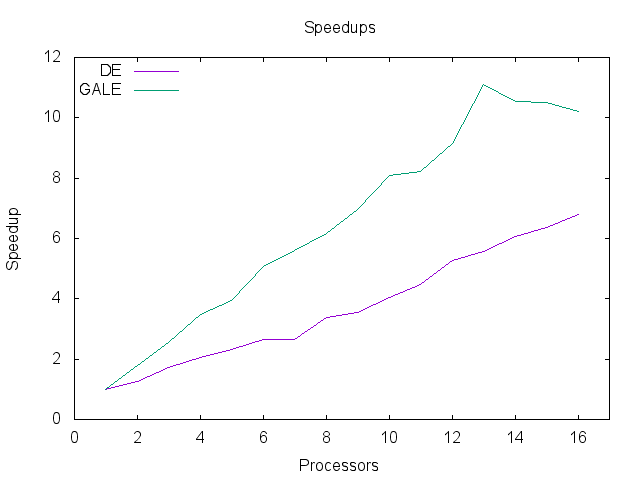
\includegraphics[width=\linewidth]{img/island/pom3/speedups}
	\end{mdframed}
	\caption{Island Model POM3 Speed Ups}	
	\label{fig:POM3_island_speedups}
    \end{minipage}
    \begin{minipage}{0.5\linewidth}
    \centering
    \begin{mdframed}
		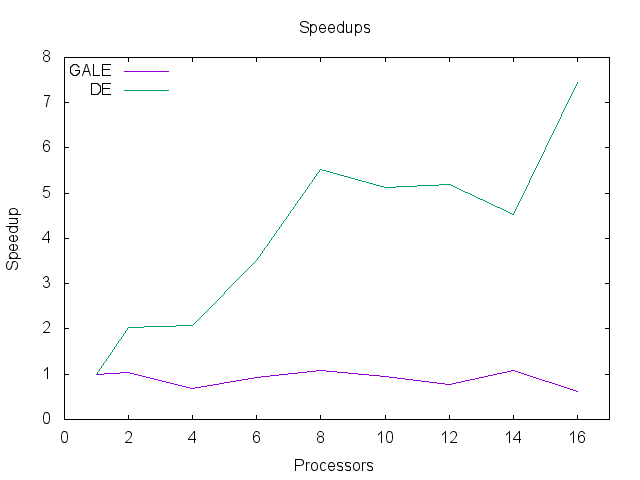
\includegraphics[width=\linewidth]{img/master-slave/pom3/speedups}
	\end{mdframed}
	\caption{Master Slave Model POM3 Speed Ups}	
	\label{fig:POM3_master_speedups}
    \end{minipage}
    \end{figure*}
	
	\clearpage
	
	\begin{figure*}[!htbp]
    \begin{minipage}{0.98\linewidth}
        \centering
        \begin{tabular}{$l@{\hspace{6pt}} $l@{\hspace{12pt}} *{9}{^c@{\hspace{10pt}}}}
        \toprule
        \rowstyle{\bfseries\boldmath} STRATEGY & \rowstyle{\bfseries\boldmath} MODEL  & 1 & 2 & 4 & 6 & 8 & 10 & 12 & 14 & 16\\
        \midrule
        \bfseries Island & \bfseries GALE
        & 229.09
        & 112.21
        & 59.90
        & 41.07
        & 30.97
        & 26.25
        & 22.37
        & 19.01 
        & 16.56 \\
        \bfseries Island & \bfseries DE
        & 8.53
        & 4.48
        & 2.33
        & 1.61
        & 1.17
        & 0.96
        & 0.77
        & 0.67
        & 0.62 \\
        \bfseries Master-Slave & \bfseries GALE
        & 86.49
        & 33.67
        & 18.16
        & 14.94
        & 13.09
        & 12.04
        & 11.69
        & 11.80
        & 10.56 \\
        \bfseries Master-Slave & \bfseries DE
        & 60.93
        & 40.12
        & 20.71
        & 14.34
        & 10.22
        & 8.21
        & 7.46
        & 6.27
        & 5.14 \\
        \bottomrule
        \end{tabular}
        \caption{Runtimes of XOMO using GALE and DE in seconds}
        \label{tab:XOMO_runtimes}
    \end{minipage}
    \begin{minipage}{0.5\linewidth}
    \centering
    \begin{mdframed}
		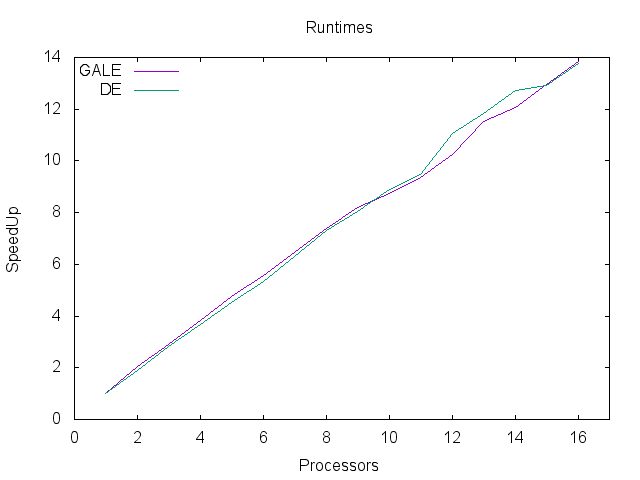
\includegraphics[width=\linewidth]{img/island/xomo/speedups}
	\end{mdframed}
	\caption{Island Model XOMO Speed Ups}	
	\label{fig:XOMO_island_speedups}
    \end{minipage}
    \begin{minipage}{0.5\linewidth}
    \centering
    \begin{mdframed}
		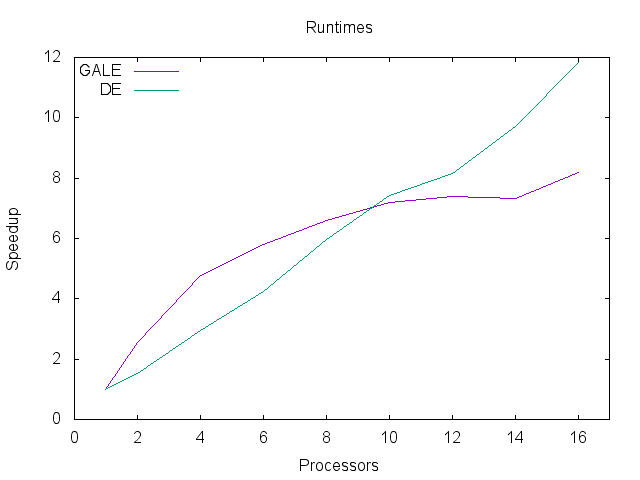
\includegraphics[width=\linewidth]{img/master-slave/xomo/speedups}
	\end{mdframed}
	\caption{Master Slave Model XOMO Speed Ups}	
	\label{fig:XOMO_master_speedups}
    \end{minipage}
    \end{figure*}
    
%     \begin{figure}
% 	\centering
%     \begin{mdframed}
% 		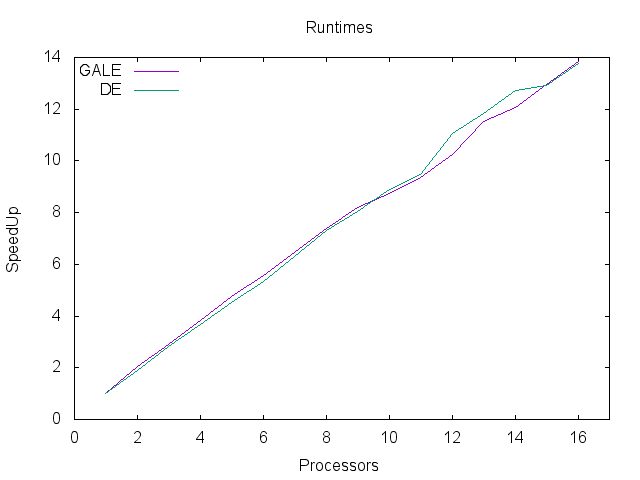
\includegraphics[width=\linewidth]{img/island/xomo/speedups}
% 	\end{mdframed}
% 	\caption{Island Model XOMO Speed Ups}	
% 	\label{fig:XOMO_island_speedups}
% 	\end{figure}
	
% 	\begin{figure}
% 	\centering
%     \begin{mdframed}
% 		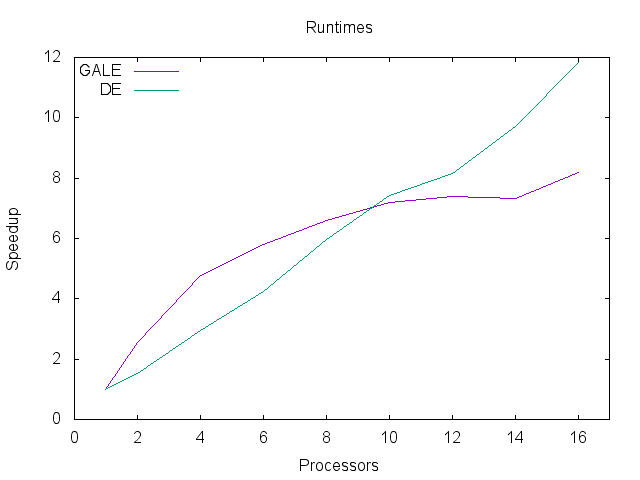
\includegraphics[width=\linewidth]{img/master-slave/xomo/speedups}
% 	\end{mdframed}
% 	\caption{Master Slave Model XOMO Speed Ups}	
% 	\label{fig:XOMO_master_speedups}
% 	\end{figure}
	
    \begin{figure*}[htbp]
    \begin{minipage}{0.98\linewidth}
        \centering
        \begin{tabular}{$l@{\hspace{6pt}} $l@{\hspace{12pt}} *{9}{^c@{\hspace{10pt}}}}
        \toprule
        \rowstyle{\bfseries\boldmath} STRATEGY & \rowstyle{\bfseries\boldmath} MODEL  & 1 & 2 & 4 & 6 & 8 & 10 & 12 & 14 & 16\\
        \midrule
        \bfseries Island & \bfseries GALE
        & 138.19
        & 65.22
        & 43.46
        & 29.26
        & 21.84
        & 18.29
        & 16.24
        & 14.47 
        & 13.97 \\
        \bfseries Island & \bfseries DE
        & 204.61
        & 103.17
        & 53.05
        & 34.65
        & 26.98
        & 29.25
        & 29.29
        & 28.64
        & 29.38 \\
        \bottomrule
        \end{tabular}
        \caption{Runtimes of ERS using GALE and DE in seconds}
        \label{tab:ERS_runtimes}
    \end{minipage}
    \noindent\hrulefill\par
    \noindent\makebox[\linewidth][c]{%
        \begin{minipage}{0.5\linewidth}
            \centering
            \begin{mdframed}
    		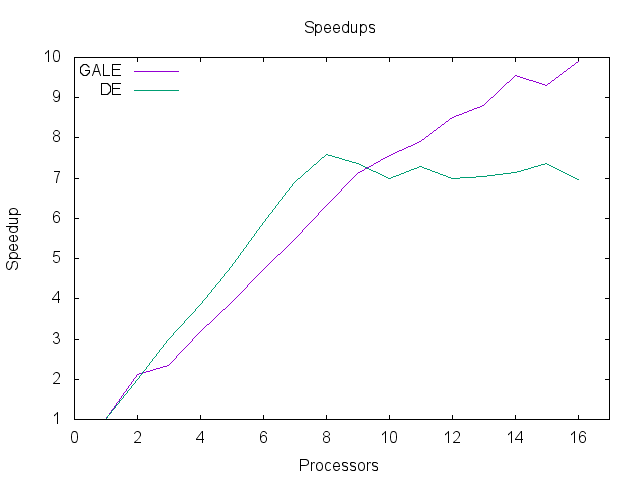
\includegraphics[width=\linewidth]{img/island/ers/speedups}
        	\end{mdframed}
        	\caption{Island Model ERS Speed Ups}	
        	\label{fig:ERS_island_speedups}
        \end{minipage}
    }
    
    
    \end{figure*}
 	\FloatBarrier
	\subsubsection{DTLZ2}
	
	
	
	The runtimes for DE and GALE on both the island and master-slave model when deployed on 1 to 16 processors is tabulated in figure \ref{tab:DTLZ2_runtimes} and speedups are shown in figures \ref{fig:DTLZ2_island_speedups} and \ref{fig:DTLZ2_master_speedups}. The results show that there is a steady increase in speedup for island model. Although, for the master slave model, GALE has significant increase in speedups, there is a plateauing effect observed for DE.
	
	\subsubsection{POM3}
	
	
    
    The runtimes for DE and GALE on both the island and master-slave model when deployed on 1 to 16 processors is tabulated in figure \ref{tab:POM3_runtimes} and speedups are shown in figures \ref{fig:POM3_island_speedups} and \ref{fig:POM3_master_speedups}. POM3 is computationally expensive and as we can see GALE outperforms DE in both the master slave and island model. In the master slave model, we observe that increasing the number of processors does not aid in better runtimes. This can be drilled down to the high communication overhead due to frequent communications in master slave over the island models.
    
	
	\subsubsection{XOMO}
	
	
    
    The runtimes for DE and GALE on both the island and master-slave model when deployed on 1 to 16 processors is tabulated in figure \ref{tab:XOMO_runtimes} and speedups are shown in figures \ref{fig:XOMO_island_speedups} and \ref{fig:XOMO_master_speedups}. XOMO is fast for a real world model and we can see that DE performs better than GALE. In the island model we observe almost exact speedups in both DE and GALE. In the master slave model we can see a plateauing effect for GALE.
    
	\subsubsection{ERS}
	
	
	
% 	\begin{figure}
% 	\centering
% 	\begin{mdframed}
% 		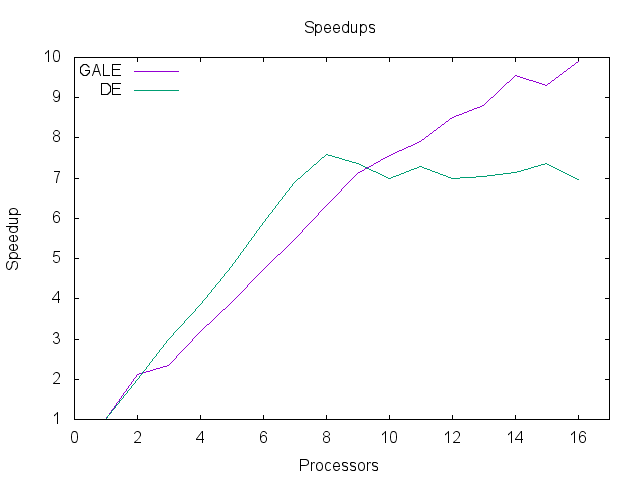
\includegraphics[width=\linewidth]{img/island/ers/speedups}
% 	\end{mdframed}
% 	\caption{Island Model ERS Speed Ups}	
% 	\label{fig:ERS_island_speedups}
% 	\end{figure}
	
	ERS was implemented only on the island model. The runtimes for DE and GALE when deployed between 1 to 16 processors is shown in Figure \ref{tab:ERS_runtimes} and the speedups are shown in \ref{fig:ERS_island_speedups}. We can see that GALE is faster than DE for this model due to the large evaluation time for GALE.
	
	\section{Conclusion}
	\label{conclusion}
	Based on our experiments we draw following conclusions:
	\begin{itemize}
	\item Parallelization strategies are effective for Multi Objective Optimization problems.
	\item For mathematical models or real world models which are not compute intensive, we suggest using Differential Evolution.
	\item For models, which require a lot of time for evaluation, we propose GALE would be optimal.
	\end{itemize}
	
	\section{Future Work}
	\label{future}
	
	This project cannot be deemed as complete but just a study on the parallelization capabilities of an MOEA. The following enhancements can be performed in the immediate future:
	\begin{enumerate}
		\item Explore mutation strategies for heavily constrained real world problems.
		\item Study these parallelization strategies for other MOEAs like NSGA2, SPEA etc.
	    \item While parallelization if we divide the feature space more effectively based on the problem space, we can achieve faster convergence to the Pareto Front. This is another avenue that can be explored.
	\end{enumerate}

    \section{Acknowledgement}
    \label{acknowledgement}
    This project is part of the course CSC 491/591 - Experimental Algorithms. We would like to thank the course staff Dr Matthias Stallmann for giving us the oppurtunity to work on this project and his constant support. We also express our gratitude to NCSU for providing us with the resources to run our experiments.
    
	\bibliographystyle{plain}
	\bibliography{refs}
\end{document}